%%%%%%%%%%%%%%%%%%%%%%%%%%%%%%%%%%%%%%%%%%%%%%%%%%%%%%%%%%%%%%%%%%%%%%%%%%%%%%%
% Chapter 2: Antecedentes
%%%%%%%%%%%%%%%%%%%%%%%%%%%%%%%%%%%%%%%%%%%%%%%%%%%%%%%%%%%%%%%%%%%%%%%%%%%%%%%

%++++++++++++++++++++++++++++++++++++++++++++++++++++++++++++++++++++++++++++++

Los capíulos intermedios servián para cubrir los siguientes aspectos:
antecedentes, problemática o estado del arte, objetivos, fases y 
desarrollo del proyecto.

En el capítulo anterior se ha introducido bla, bla, bla ....

%++++++++++++++++++++++++++++++++++++++++++++++++++++++++++++++++++++++++++++++

\section{SIMDE}
\label{2:sec1}

En el año dos mil cuatro, el por aquel entonces estudiante de esta universidad, 
Iván Castilla Rodríguez - y ahora tutor de este trabajo de fin de grado-, 
desarrolló como proyecto final de carrera un Simulador didáctico para la enseñanza 
de arquitectura de computadores, el cual fue bautizado como Simde. 

\bigskip
Este simulador como se ha comentado en el apartado 1.4 cumple con las características
deseadas y esperadas de un simulador para la docencia de este ámbito.

\bigskip
Sin embargo, esta herramienta ya se encuentra desfasada. No ha sido un proyecto en constante
evolución, fue hecha utilizando C++98 y C++ Builder y necesita un nuevo enfoque.

\begin{figure}[!th]
\begin{center}
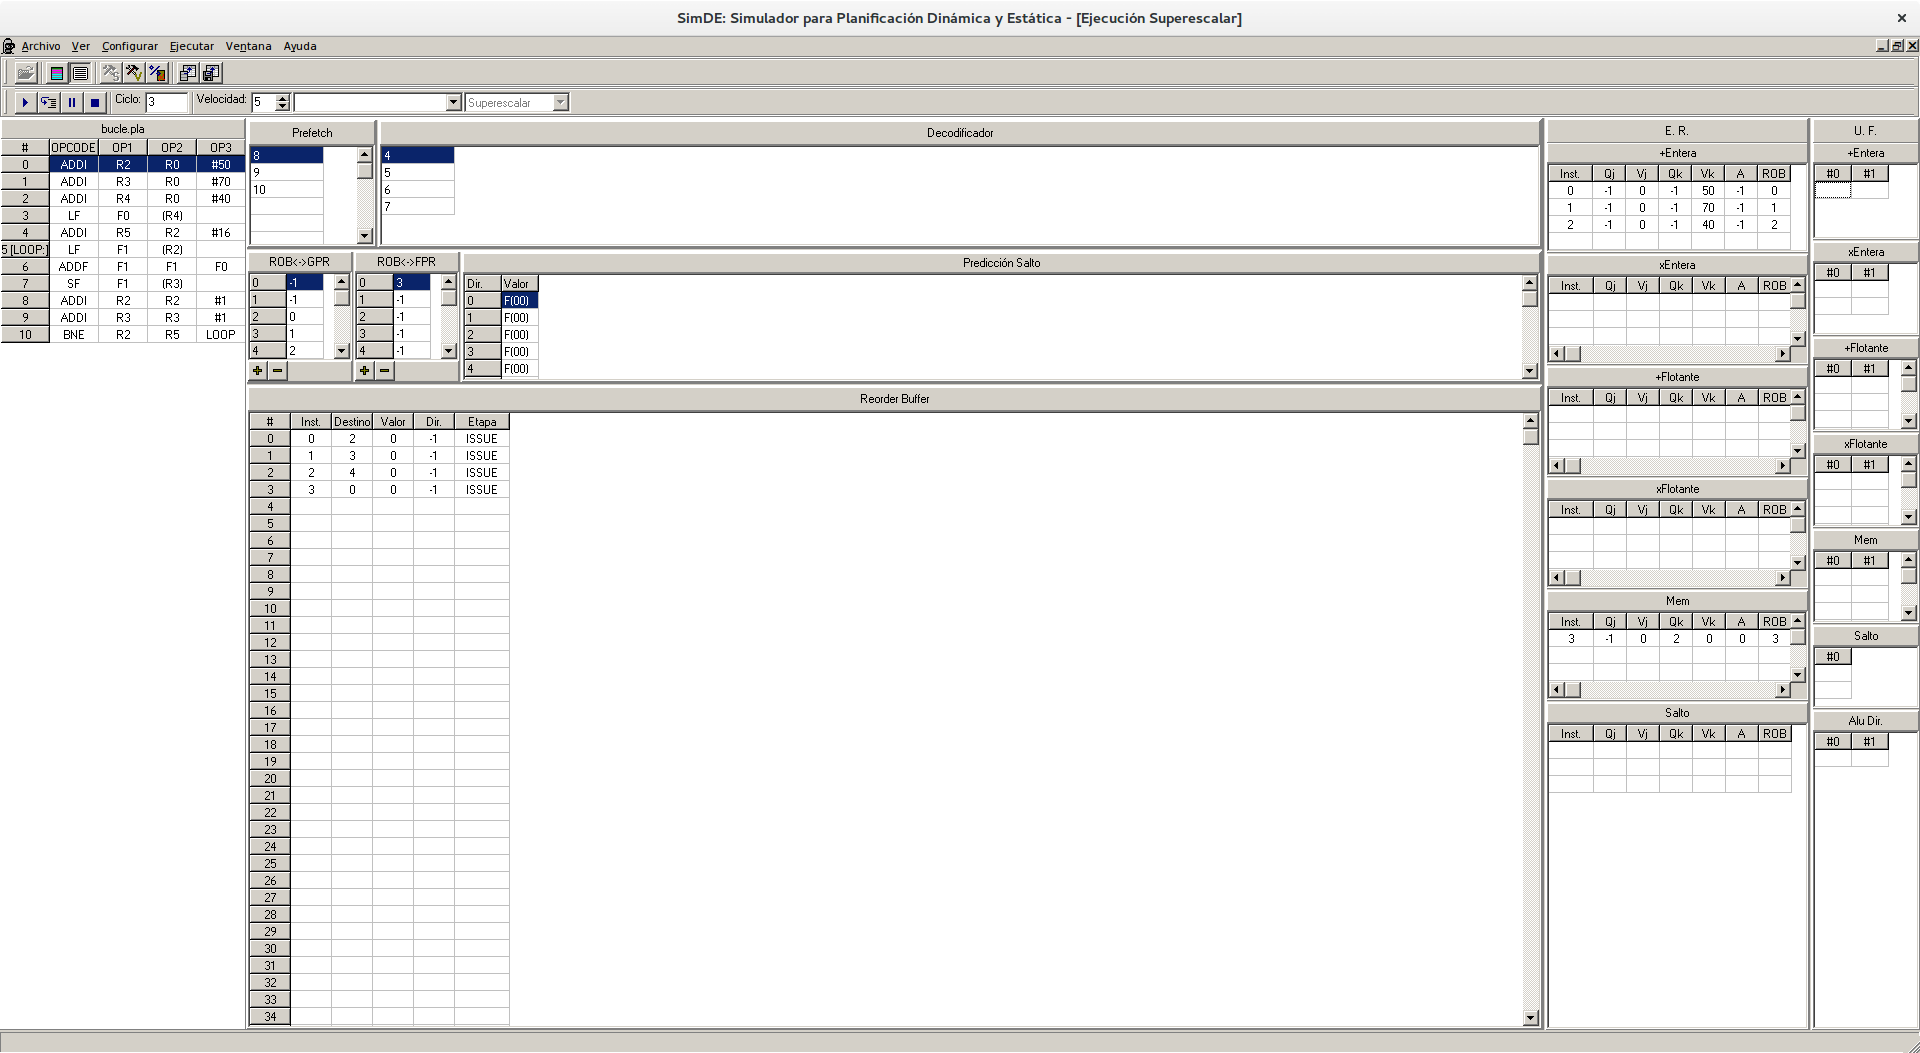
\includegraphics[width=0.8\textwidth]{images/cap2/simdeoriginal.eps}
\caption{Emulador original de SIMDE}
\label{fig:Emulador original de SIMDE}
\end{center}
\end{figure}

A día de hoy, una de las mejores soluciones para implementar este tipo de simulador es la web.
Permitiendo la accesibilidad por un mayor número de usuarios, centralizando el acceso a la 
aplicación y sobre todo, explotando todas las nuevas herramientas que se han ido generando
con el paso del tiempo.

\section{Otros simuladores}
\label{2:sec2}

Sería irrazonable embarcarse en la tarea de migrar SIMDE. 

